\chapter{Scripting 2}

\begin{summary}
This chapter is build upon the previous one and continues to explore more advanced scripts and techniques for locking and unlocking funds in the Bitcoin network. Several examples are provided.
\end{summary}

\section{Timelocks}
Timelocks is a mechanism for postdating transactions or to lock funds for specific periods of time. It applies only to version 2 transactions. There are two different types of locking, one for absolute and one for relative time. In each one we can specify timelocks at transaction level or at script level. 

\subsection*{Absolute at transaction level}
This feature was part of the initial Bitcoin implementation. Every transaction can include a timelock (\keyword{nLocktime}) to specify the earliest time that a transaction may be added to a block. Wallets were setting this value to \keyword{0} meaning that the transaction is valid anytime. Later on, a soft-fork allowed to specify the time in terms of the block height. Possible values:

\begin{table}[h]
\centering
\begin{tabular}[H]{ |L{0.27\linewidth}|L{0.67\linewidth}| }
\hline
0 & Transaction is always valid.\\
\hline
< 500 million & Specifies the earliest block height that this transactions can be added.\\
\hline
>= 500 million & Specifies the block header time (Unix Epoch) after which the transaction can be added to a block.\\
\hline
\end{tabular}
\end{table}

Absolute \keyword{nLocktime} is used in some wallets to prevent fee sniping. Fee sniping is a theoretical attack that involves large miners/pools mining two (or possibly more) blocks in an attempt to reorganize past blocks. The miner can then add the highest-fee transactions from the previously valid blocks plus any high-fee transactions in the mempool.

The Bitcoin Core wallet (from 0.11.0) creates transactions that include an \keyword{nLocktime} of the current best height plus one. Thus, the transaction is valid for the next block as normal but in the case of a reorg a miner cannot add this transaction in a previous block. This means that, if all transactions use this mechanism, the miner will not be able to gain any new fees by including new transactions to older blocks.
This will be more important as the miners' reward is reduced further making transaction fees the major source of income for miners.

This can be achieved by setting \keyword{nLocktime} and \keyword{nSequence} appropriately.

\begin{emphbox}
\begin{lstlisting}[style=Pseudomath]
nLocktime = current_best_height + 1
nSequence = 0xFFFFFFFE
\end{lstlisting}
\end{emphbox}

The original idea behind \keyword{nSequence} was that a transaction in the mempool would be replaced by using the same input with a higher sequence value. This assumes that miners would prefer higher sequence number transactions instead of more profitable ones (i.e. higher fee) which would never work. 

For this reason the \keyword{nSequence} input field was repurposed to specify additional transaction semantics like timelocks. Typical transactions have an \keyword{nSequence} of \keyword{0xFFFFFFFF}.

For example, as we can see in figure~\ref{fig:absolute-timelock}, if we want to spent a UTXO of transaction $TX_{x}$ in block $Y$ (a block in the future, say 700000) we need to create a transaction that spends it but also set \keyword{nLocktime} to $Y$. Then this new transaction $TX_{x+1}$ will be invalid until that block height.

\vspace{0.5em}
\begin{figure}[H]
\begin{center}
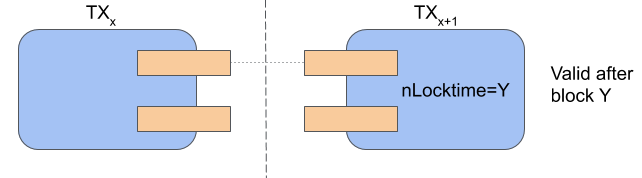
\includegraphics[scale=0.6]{images/absolute-timelock}
\caption{Example: absolute timelock.}
\label{fig:absolute-timelock}
\end{center}
\end{figure}

Note that nLocktime creates a transaction that cannot be included in the blockchain until the specified block/time. This means that the person who created the transaction could create another transaction to spend the funds, invalidating the nLocktime transaction. This is problematic in several use cases and thus absolute timelocks at script level were created.


\subsection*{Absolute at script level}
Absolute locktime is achieved at the script level using the \keyword{CHECKLOCKTIMEVERIFY} or \emph{CLTV} opcode. In late 2015 the BIP-65\footnote{https://github.com/bitcoin/bips/blob/master/bip-0065.mediawiki} soft-fork redefined \keyword{OP\_NOP2}\footnote{A \emph{no-operator} operator does nothing and is reserved to add future functionality.} as \keyword{OP\_CHECKLOCKTIMEVERIFY} allowing timelocks to be specified per transaction output. To spent the output, the signature and public key are required as usual but the nLocktime field of the spending transaction also needs to be set to an equal or greater value of CLTV’s timelock value. If not the script will fail immediately.

A \keyword{scriptPubKey} example that locks an output until an \keyword{expiry\_time} \emph{and} a P2PKH equivalent would look like:

\begin{emphbox}
\begin{verbatim}
<expiry_time> OP_CHECKLOCKTIMEVERIFY OP_DROP 
OP_DUP OP_HASH160 <PKHash> OP_EQUALVERIFY OP_CHECKSIG
\end{verbatim}
\end{emphbox}

To spend a transaction output with a timelock we need to specify the future block in \keyword{nLocktime} and activate the \keyword{nSequence} of the particular input that we want to spend to \keyword{0xFFFFFFFE}.

\begin{note}
Since a script with \keyword{CHECKLOCKTIMEVERIFY} becomes part of the blockchain it cannot be invalidated as described above with the transaction-level equivalent. 
\end{note}

For example, as we can see in figure~\ref{fig:script-absolute-timelock} we can create a locking script with CLTV on block $Y$ (a block in the future, say 700000) and send some funds to it (and keep sending). If we want to spend it we need to create a transaction that spends it but also sets \keyword{nLocktime} to at least 700000. Then this new transaction $TX_{x+1}$ will be invalid until that block height.

\vspace{0.5em}
\begin{figure}[H]
\begin{center}
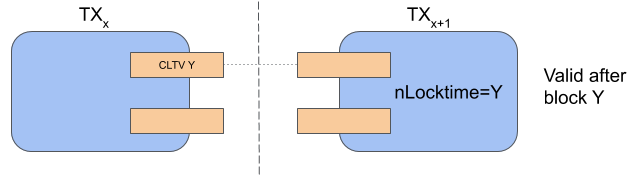
\includegraphics[scale=0.6]{images/script-absolute-timelock}
\caption{Example: script-level absolute timelock.}
\label{fig:script-absolute-timelock}
\end{center}
\end{figure}


\subsection*{Relative at transaction input level}
Relative timelocks where introduced in mid-2016 with BIPs 68\footnote{https://github.com/bitcoin/bips/blob/master/bip-0068.mediawiki} and 113\footnote{https://github.com/bitcoin/bips/blob/master/bip-0113.mediawiki} as a soft-fork that made use of the \keyword{nSequence} field of an input. 

\keyword{nSequence} was repurposed for relative timelocks. If the most significant bit of the \keyword{nSequence} 32-bit field was \keyword{0} (i.e. \keyword{0x7FFFFFFF}) then it was interpreted as a relative timelock. Then, for timelocks bit 23 would specify the type (block height or Unix Epoch time) and the last 16 bits the value.

\begin{table}[h]
\centering
\begin{tabular}[H]{ |L{0.27\linewidth}|L{0.67\linewidth}| }
\hline
\textbf{Type (bit 23)} & \textbf{Meaning of last (least significant) 16 bits}\\
\hline
0 & The number of blocks that need to pass based on the height of the UTXO which the input spends.\\
\hline
1 & The number of 512 seconds intervals that need to pass based on the timestamp of the UTXO which the input spends.\\
\hline
\end{tabular}
\end{table}

For example, as shown in figure~\ref{fig:relative-timelock}, if we want to spent a UTXO of transaction $TX_{x}$ after 10 blocks we need to create a transaction that spends it but also set \keyword{nSequence} to 10. Then this new transaction $TX_{x+1}$ will be invalid until $TX_{x}$ gets 10 confirmations.

\vspace{0.5em}
\begin{figure}[H]
\begin{center}
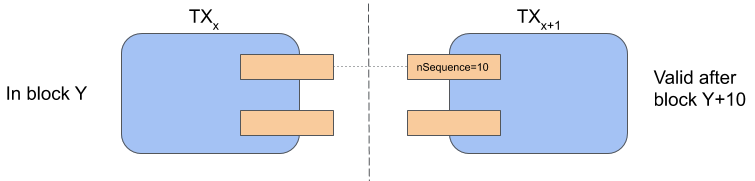
\includegraphics[scale=0.6]{images/relative-timelock}
\caption{Example: relative timelock.}
\label{fig:relative-timelock}
\end{center}
\end{figure}


\subsection*{Relative at script level}
The script-level equivalent of relative timelocks is using \keyword{CHECKSEQUENCEVERIFY} or \emph{CSV} defined in BIP-112\footnote{https://github.com/bitcoin/bips/blob/master/bip-0112.mediawiki}. It replaces \keyword{OP\_NOP3} with \keyword{OP\_CHECKSEQUENCEVERIFY}. When we create a transaction that spends a UTXO that contains a CSV, that input requires to have \keyword{nSequence} set with an equal or greater value to the CSV parameter value. Otherwise it will fail immediately.

Expiry date can be expressed in either block height or timestamp (as previously discussed) but it has to be the same type as the one used in the \keyword{nSequence} field. Note that in the script only the block height or timestamp is included\footnote{If timestamp the 23rd bit has to exist and be set. Also note that integers in the script should be serialized as signed integers in little-endian. Fortunately, programming libraries hide these details from the developers.} and not the whole \keyword{nSequence} field.

For example, we can create a locking script with CSV with a value of 10 blocks and send some funds to it (and keep sending). If we want to spend it we need to create a transaction that spends it but also set the \keyword{nSequence} of the input that spends it to 10. Then, this new transaction $TX_{x+1}$ will be invalid until $TX_{x}$ gets 10 confirmations.

\vspace{0.5em}
\begin{figure}[H]
\begin{center}
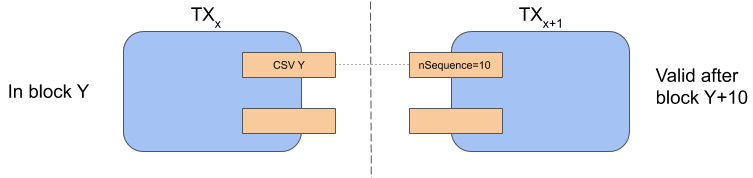
\includegraphics[scale=0.6]{images/script-relative-timelock}
\caption{Example: script-level relative timelock.}
\label{fig:script-relative-timelock}
\end{center}
\end{figure}


\subsection*{Timelock types summary}

\begin{table}[h]
\centering
\begin{tabular}[H]{ |C{0.12\linewidth}|C{0.13\linewidth}|C{0.12\linewidth}|C{0.12\linewidth}|L{0.38\linewidth}| }
\hline
\textbf{Type} & \textbf{Location} & \textbf{Time specification} & \textbf{In blockchain} & \textbf{Example}\\
\hline
nLocktime & Transaction & Absolute & No & Similar to a will. Your heirs could get the funds in ~2040 but you could spend them (changle will) in between.\\
\hline
nLocktime + CLTV & Script & Absolute & Yes & Lock funds as part of a deal that allows no one access until ~1-Jan-2020. Used in CLTV-based payment channels.\\
\hline
nSequence & Input & Relative & No & Lock funds as part of a deal that prohibits the other party to spend funds until ~3 months have passed but you can.\\
\hline
nSequence + CSV & Script & Relative & Yes & Lock funds as part of a deal that allows no one access until ~3 months have passed. Used in payment channels and Lightning network\\
\hline
\end{tabular}
\end{table}



\subsection*{Example: create a P2SH address with a relative timelock}
\label{ssec:p2sh-csv-address-example}
Since the script we are going to create is not standard we need to wrap it using a P2SH output. Any funds send to that address will be locked for 20 blocks as well as with an P2PKH-equivalent script. The example is borrowed from \keyword{python-bitcoin-utils}\footnote{https://github.com/karask/python-bitcoin-utils/blob/master/examples/create\_p2sh\_csv\_p2pkh\_address.py}.

\vspace{1em}
\begin{lstlisting}[style=Python]
from bitcoinutils.setup import setup
from bitcoinutils.transactions import Transaction, TxInput, TxOutput, Sequence
from bitcoinutils.keys import P2pkhAddress, P2shAddress, PrivateKey
from bitcoinutils.script import Script
from bitcoinutils.constants import TYPE_RELATIVE_TIMELOCK

def main():
    # always remember to setup the network
    setup('testnet')

    # This script creates a P2SH address containing a CHECKSEQUENCEVERIFY plus
    # a P2PKH; locking funds with a key as well as for 20 blocks

    # set values
    relative_blocks = 20

    seq = Sequence(TYPE_RELATIVE_TIMELOCK, relative_blocks)

    # secret key corresponding to the pubkey needed for the P2SH (P2PKH) transaction
    p2pkh_sk = PrivateKey('cRvyLwCPLU88jsyj94L7iJjQX5C2f8koG4G2gevN4BeSGcEvfKe9')

    # get the address (from the public key)
    p2pkh_addr = p2pkh_sk.get_public_key().get_address()

    # create the redeem script
    redeem_script = Script([seq.for_script(), 'OP_CHECKSEQUENCEVERIFY', 'OP_DROP', 
                           'OP_DUP', 'OP_HASH160', p2pkh_addr.to_hash160(),
                           'OP_EQUALVERIFY', 'OP_CHECKSIG'])

    # create a P2SH address from a redeem script
    addr = P2shAddress.from_script(redeem_script)
    print(addr.to_string())

if __name__ == "__main__":
    main()
\end{lstlisting}
\vspace{1em}



\subsection*{Example: spend funds from a P2SH timelocked address}
\label{ssec:p2sh-csv-spend-example}
Assuming that someone has sent funds to the P2SH address that we created above we can use this program to spend it. As usual and for simplicity, values are hard-coded and no change outputs are specified. The example is borrowed from \keyword{python-bitcoin-utils}\footnote{https://github.com/karask/python-bitcoin-utils/blob/master/examples/spend\_p2sh\_csv\_p2pkh.py}.

\vspace{1em}
\begin{lstlisting}[style=Python]
from bitcoinutils.setup import setup
from bitcoinutils.utils import to_satoshis
from bitcoinutils.transactions import Transaction, TxInput, TxOutput, Sequence
from bitcoinutils.keys import P2pkhAddress, P2shAddress, PrivateKey
from bitcoinutils.script import Script
from bitcoinutils.constants import TYPE_RELATIVE_TIMELOCK

def main():
    # always remember to setup the network
    setup('testnet')

    # We assume that some 11.1 tBTC have been send to that address and that we know
    # the txid and the specific UTXO index (or vout).

    # set values
    relative_blocks = 20
    txid = '76c102821b916a625bd3f0c3c6e35d5c308b7c23e78b8866b06a3a466041db0a'
    vout = 0

    seq = Sequence(TYPE_RELATIVE_TIMELOCK, relative_blocks)

    # create transaction input from tx id of UTXO (contained 11.1 tBTC)
    txin = TxInput(txid, vout, sequence=seq.for_input_sequence())

    # secret key needed to spend P2PKH that is wrapped by P2SH
    p2pkh_sk = PrivateKey('cRvyLwCPLU88jsyj94L7iJjQX5C2f8koG4G2gevN4BeSGcEvfKe9')
    p2pkh_pk = p2pkh_sk.get_public_key().to_hex()
    p2pkh_addr = p2pkh_sk.get_public_key().get_address()

    # create the redeem script - needed to sign the transaction
    redeem_script = Script([seq.for_script(), 'OP_CHECKSEQUENCEVERIFY', 'OP_DROP',
                           'OP_DUP', 'OP_HASH160', p2pkh_addr.to_hash160(),
                           'OP_EQUALVERIFY', 'OP_CHECKSIG'])

    # to confirm that address is the same as the one that the funds were sent
    #addr = P2shAddress.from_script(redeem_script)
    #print(addr.to_string())

    # send/spend to any random address
    to_addr = P2pkhAddress('n4bkvTyU1dVdzsrhWBqBw8fEMbHjJvtmJR')
    txout = TxOutput(to_satoshis(11), to_addr.to_script_pub_key() )

    # no change address - the remaining 0.1 tBTC will go to miners)

    # create transaction from inputs/outputs
    tx = Transaction([txin], [txout])

    # print raw transaction
    print("\nRaw unsigned transaction:\n" + tx.serialize())

    # use the private key corresponding to the address that contains the
    # UTXO we are trying to spend to create the signature for the txin -
    # note that the redeem script is passed to replace the scriptSig
    sig = p2pkh_sk.sign_input(tx, 0, redeem_script )

    # set the scriptSig (unlocking script) -- unlock the P2PKH (sig, pk) plus
    # the redeem script, since it is a P2SH
    txin.script_sig = Script([sig, p2pkh_pk, redeem_script.to_hex()])
    signed_tx = tx.serialize()

    # print raw signed transaction ready to be broadcasted
    print("\nRaw signed transaction:\n" + signed_tx)
    print("\nTxId:", tx.get_txid())


if __name__ == "__main__":
    main()
\end{lstlisting}
\vspace{1em}


\subsection*{Timelocks important caveat}
\label{ssec:timelocks-important-caveat}
Remember that \keyword{nLockTime} is set for the whole transaction and that it is either specified as a block height or as block header time (Unix Epoch). Thus, if the transaction tries to spend two inputs one with block height CLTV and the other with time CLTV it would be impossible to spend. 
\begin{emphbox}
\begin{lstlisting}[style=Pseudomath]
Input 0:
	1 OP_CLTV
Input 1:
	500000001 OP_CLTV
\end{lstlisting}
\end{emphbox}

The same would apply even for a single locking script that had both types of absolute locking.

\begin{emphbox}
\begin{lstlisting}[style=Pseudomath]
1 OP_CLTV OP_DROP 500000001 OP_CLTV
\end{lstlisting}
\end{emphbox}

Relative timelocks use \keyword{nSequence} which is per input and thus for CSV the issue comes up only when a single script has both types of locking.



\section{RBF \& CPFP}
\emph{Replace-by-fee} and \emph{child-pays-for-parent} are two mechanisms that can help when transactions are stuck in the mempool due to low fees. They probably don't belong to the scripting section but RBF uses \keyword{nSequence}, the values of which, could influence timelocks. 

\subsection*{Replace-By-Fee}
Replace-by-fee, specified in BIP-125\footnote{https://github.com/bitcoin/bips/blob/master/bip-0125.mediawiki} is a mechanism for replacing any transaction that is still in the mempool. It is primarily useful for re-sending a transaction of yours in case it was stuck, e.g. due to low fees. However, it may be useful for other reasons.

Similar to timelocks it applies only to version 2 transactions and you need to set \keyword{nSequence} to a value of \keyword{0x01} to \keyword{0x7fffffff}. However, since that such a value also enables relative timelocks one has to be careful. Typically, for RBF you set the \keyword{nSequence} value to \keyword{1}, which makes relative timelocks irrelevant, or from \keyword{0xf0000000} to \keyword{0xfffffffd} which disables relative timelocks.

When creating transactions with the Bitcoin core software RBF transactions are opt-in. A replaceable transaction has the \keyword{bip125-replaceable} flag set to \keyword{yes} in its JSON display. You can make all transactions replaceable by default by setting \keyword{walletrbf=1} as a node option.

To work, in addition to setting the \keyword{nSequence} the transaction needs to reuse one or more of the same UTXOs\footnote{Note that this allows the new transaction to have different output addresses.} and increase the fees.

Using the Bitcoin core wallet there is an easy way to RBF a transaction (that is, of course, replaceable) by using \keyword{bumpfee}:

\begin{emphbox}
\begin{lstlisting}[style=Bash]
$ bitcoin-cli -named bumpfee txid=53fe...ffb4
\end{lstlisting}
\end{emphbox}


\subsection*{Child-pays-for-parent}
Child-pays-for-parent or CPFP is a mechanism (or trick, if you wish) for including a previous transaction (parent) in a block by creating a transaction (child) that spends one of the UTXOs of the parent. Miners will notice that the new transaction uses another one and will consider both transactions' fees when deciding whether to include it in the next block.

For example if someone sends you bitcoins but the transaction was stuck (e.g. due to low fees) you as a recipient can create a transaction that tries to spend the bitcoins from your address from the unconfirmed transaction. The fees of this transaction should be quite high to properly incentivize the miner (i.e. proper fees for two transactions).

If the fee is high enough the miner will want to include the new (child) transaction and in doing so he is forced to include the initial transaction (parent) in the same block.
There is nothing special with CPFP and can apply to any transaction. It makes use of miners' incentives to prioritize a transaction.

\begin{note}
The \emph{sender} of some funds can use RBF to increase the fee to unstuck a transaction from the mempool. The \emph{recipient} of some funds can use CPFP to indirectly increase the fee to unstuck a transaction from the mempool.
\end{note}



\section{Hash Time-Locked Contracts}
\label{sec:htlc}

\subsection*{Hashlocks}
A hashlock is a type of locking script that restricts the spending of an output until a specific piece of data, e.g. a passphrase, is publicly revealed. The passphrase can be shared by any means. All hashlock outputs using the same passphrase can then be spent. Such a locking script would be:

\begin{emphbox}
\begin{lstlisting}[style=Pseudomath]
OP_HASH256 <passphrase_hash> OP_EQUAL
\end{lstlisting}
\end{emphbox}

This makes it possible to create multiple outputs locked with the same hashlock and when one is spent the rest will also be available for spending, since, by spending one the passphrase will be revealed). Effectively, by spending one such output you share the passphrase.

Of course, since the passphrase will become public, everyone will be able to spend the rest of the outputs, which is not very useful. Thus, outputs protected by hashlocks are typically also protected by specific signatures so that only the owners of the corresponding keys could spend the remaining outputs. This is similar to what 2FA offers (something one owns and something one knows).

\begin{emphbox}
\begin{lstlisting}[style=Pseudomath]
OP_HASH256 <passphrase_hash> OP_EQUALVERIFY 
OP_DUP OP_HASH160 <PKHash> OP_EQUALVERIFY OP_CHECKSIG
\end{lstlisting}
\end{emphbox}


\subsection*{HTLC}
\label{ssec:htlc}
A \emph{Hashed Time-Locked Contract} (BIP-199\footnote{https://github.com/bitcoin/bips/blob/master/bip-0199.mediawiki}) is a combination of a hashlock and a timelock that requires the receiver of a payment to either provide a passphrase or forfeit the payment allowing the sender to take the funds back. For example:

\begin{emphbox}
\begin{lstlisting}[style=Pseudomath]
OP_IF
    OP_SHA256 <passphrase_hash> OP_EQUALVERIFY 
    OP_DUP OP_HASH160 <receiver PKH>
OP_ELSE
    100 OP_CHECKSEQUENCEVERIFY OP_DROP 
    OP_DUP OP_HASH160 <sender PKH>
OP_ENDIF
OP_EQUALVERIFY
OP_CHECKSIG
\end{lstlisting}
\end{emphbox}

The above locking script would be created by both sender and receiver collaborating. The receiver knows the passphrase, also called \emph{pre-image}, but only shares its hash, also called \emph{digest}. The sender can then send some funds to that P2SH address. The receiver can claim the funds if he reveals (in the blockchain) the passphrase. If not, after 100 blocks pass the sender can claim the funds.

Let's go through this scenario in more detail. Alice wants to learn some information, e.g. a passphrase, and is willing to pay to get it. Bob has the passphrase and is willing to \emph{sell} it\footnote{This scenario might sound very abstract but it will make more sense in the Atomic Swaps section.}. To setup an HTLC, see figure~\ref{fig:htlc} (i), the following steps are required:

\begin{itemize}
\item Alice (sender) and Bob (receiver) exchange public keys
\item Alice and Bob agree upon a timeout threshold
\item Bob sends the \keyword{passphrase\_hash} (digest) to Alice
\item They can now both create the script and P2SH address
Alice sends funds to the new P2SH address
\end{itemize}

\begin{figure}[h]
\begin{center}
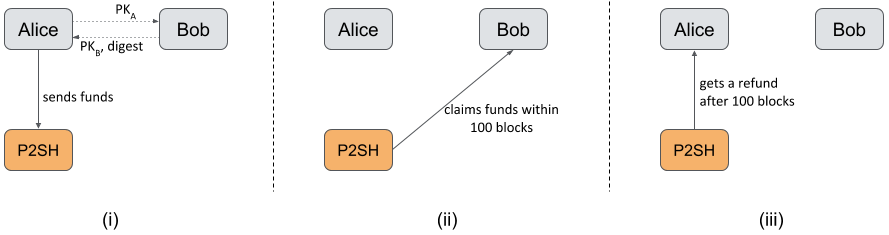
\includegraphics[scale=0.5]{images/htlc}
\caption{HTLC setup with potential scenarios.}
\label{fig:htlc}
\end{center}
\end{figure}

According to the locking script there are only two possible scenarios as seen in figure~\ref{fig:htlc} (ii) and (iii) respectively.
\begin{enumerate}[(i)]
\setcounter{enumi}{1}
\item Bob claims the funds and in doing so reveals the passphrase.
\item Bob does not claim the funds until the agreed timeout. Alice can take the funds back.
\end{enumerate}

\subsection*{HTLC Applications}
HTLC transactions are a safe and cheap method of exchanging secrets for money over the blockchain. Applications include Atomic Swaps, Lightning Network, Zero-knowledge contingent payments\footnote{https://bitcoincore.org/en/2016/02/26/zero-knowledge-contingent-payments-announcement/} and potentially several others.



\section{Atomic Swaps}
\label{sec:atomic-swaps}
Atomic Swaps is a way of trustlessly exchanging funds between different blockchains. You can swap funds in a predetermined exchange rate. For example Alice wants to send 1 BTC to Bob in the Bitcoin blockchain and receive 100 LTC from Bob in the Litecoin blockchain. It is important that these two transactions \emph{effectively} happen atomically, either both happen or none.

To accomplish that we can use two HTLC contracts, one in each blockchain. The same passphrase should be used, thus once the funds from one of the blockchains is claimed (passphrase revealed) it can immediately be claimed in the other.

Let us describe a step-by-step example demonstrating the mechanism as seen in figure~\ref{fig:atomic-swap}.

\begin{figure}[h]
\begin{center}
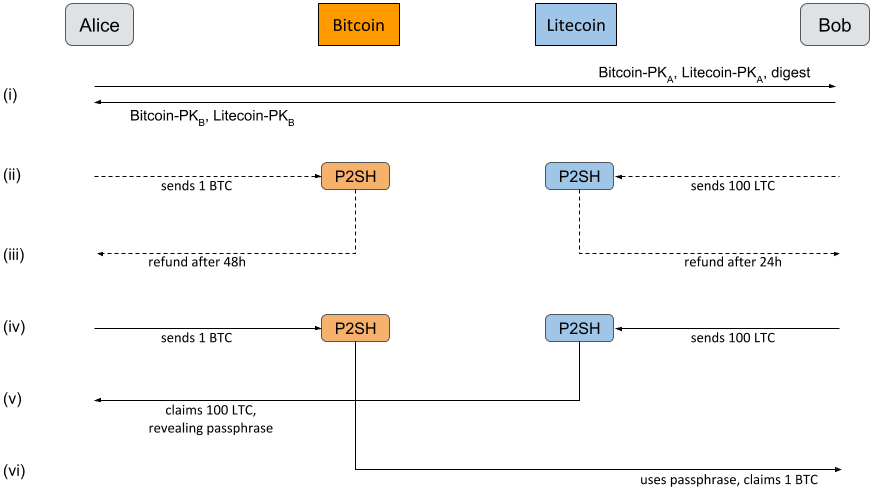
\includegraphics[scale=0.5]{images/atomic-swap}
\caption{Atomic swap between Bitcoin and Litecoin blockchains.}
\label{fig:atomic-swap}
\end{center}
\end{figure}

\begin{enumerate}[(i)]
\item Initial setup
  \begin{itemize}
  \item Alice and Bob exchange public keys on both Bitcoin and Litecoin.
  \item Alice and Bob agree upon the timeout thresholds, say 48 and 24 hours.
  \item Alice knows of a passphrase (pre-image) which is hashed to produce a digest; the latter is shared with Bob.
  \end{itemize}

\item Both Alice and Bob create a HTLC for the Bitcoin and Litecoin blockchain respectively. The funds can be redeemed by:
  \begin{itemize}
  \item the passphrase and their counterpart's signature, or
  \item by both Alice's and Bob's signatures.
  \item Alice sends 1 BTC to the Bitcoin's HTLC and Bob sends 100 LTC to the Litecoin's HTLC. \emph{No one} broadcasts the transaction!
  \end{itemize}

\item Both Alice and Bob create a refund transaction for the funds they have just sent
  \begin{itemize}
  \item Alice creates a timelocked refund transaction that would be valid after 48 hours.
  \item Bob creates a timelocked refund transaction that would be valid after 24 hours.
  \item Both pass the refund transaction to their counterpart for their signature (satisfying the ``both signatures'' clause of the HTLCs).
  \item They now both have a final refund transaction that is ready to be broadcasted if something goes wrong.
  \end{itemize}

\item Alice and Bob both broadcast the funding transaction from step (ii).

\item Alice unlocks the Litecoin HTLC by the ``passsphrase'' clause of the HTLC revealing the passphrase in the process.

\item Bob uses the passphrase to unlock the Bitcoin HTLC as well and the atomic swap was successful.

\end{enumerate}

Note that the above ordering is not strict in any sense. As long as the refund transactions are both signed before the passphrase is revealed everyone is safe.

If Bob does not send the LTC, Alice will be able to get her 1 BTC back after 48 hours by broadcasting her refund transaction.

If Alice does not send the BTC, Bob will be able to get his 100 LTC back after 24 hours by broadcasting his refund transaction.

It is important to understand that active participation is required in this exchange. For example, if Bob does not use the passphrase to claim the bitcoin in time after the passphrase is revealed, Alice can use her refund transaction and also get her bitcoin back! 

\begin{note}
Participants in an atomic swap need to inspect the blockchain for the relevant transactions!
\end{note}

Atomic swaps allow for trustless exchange between assets of different blockchains. One potential use case is trustless decentralized exchanges. 




\section{Payment Channels}
\label{sec:payment-channels}
Payment channels is a class of techniques that allows two participants to make multiple Bitcoin transactions without committing all of those transactions to the blockchain; i.e. most of the transactions are off-chain.

The Bitcoin wiki lists\footnote{https://en.bitcoin.it/wiki/Payment\_channels} several approaches to implement Payment Channels. We will only go through some of them including the one currently used in the Lightning Network.

\begin{itemize}
\item Nakamoto high-frequency transactions
\item \textbf{Spillman-style payment channels}
\item \textbf{CLTV-style payment channels}
\item \textbf{Poon-Dryja payment channels}
\item Decker-Wattenhofer duplex payment channels
\item Decker-Russell-Osuntokun eltoo Channels (eltoo; requires SIGHASH\_INPUT)
\end{itemize}


\subsection*{Spillman-style payment channels}
TODO


\subsection*{CLTV-style payment channels}
TODO


\subsection*{Poon-Dryja payment channels}
TODO




\section{Exercises}

\begin{exercise}
In section~\ref{ssec:p2sh-csv-address-example} we created an address for a relative timelock. Now create an address that locks the funds with an absolute timelock some time in the future (use block height or timestamp).
\end{exercise}

\begin{exercise}
In section~\ref{ssec:p2sh-csv-spend-example} we spent from an address with a relative timelock. Now create a script that unlocks the funds from an address with an absolute timelock like the one created in the previous exercise.
\end{exercise}

\begin{exercise}
Implement the example HTLC scenario of section~\ref{ssec:htlc}. Create the appropriate scripts for both Alice and Bob.
\end{exercise}

\begin{exercise}
Write the HTLC locking script that Alice needs to write for the atomic swap in step (ii) as described in section~\ref{sec:atomic-swaps}. 
\end{exercise}

\begin{exercise}
Write the unlocking script that Alice needs to use to claim the litecoin in step (v) as described in section~\ref{sec:atomic-swaps}. 
\end{exercise}

\begin{exercise}
Try to design a platform that would facilitate atomic swaps between Bitcoin and Litecoin. Think about it holistically and in practical terms; i.e. how would you design and implement such a platform. Keep a note of all the potential difficulties that might come up and try to find solutions.
\end{exercise}



